\section[Desenvolvimento do Projeto]{Desenvolvimento do Projeto}

\subsection{Metodologia de Desenvolvimento}
  O desenvolvimento do projeto é organizado em Sprints de duas semanas, seguindo os princípios da metodologia Scrum \cite{scrum}, conforme proposto pela \acs{ages}. Nossa equipe está inserida em uma estrutura de squads, onde cada um é liderado por um colega de \acs{ages} III e composto por alunos de \acs{ages} I e II, o que permite um trabalho mais focado e colaborativo.

  Cada Sprint se inicia com uma cerimônia de Planejamento (Sprint Planning), momento em que os colegas \acs{ages} IV apresentam as User Stories e as tarefas são distribuídas entre as equipes.

  Para garantir o alinhamento contínuo durante a execução da Sprint, adotamos uma rotina de sincronização diária. Durante as aulas presenciais de terça e quinta-feira, realizamos uma Daily Scrum, na qual o andamento das tarefas registradas no Azure DevOps \cite{azuredevops} é revisado. Nos demais dias, essa sincronização ocorre de forma assíncrona por meio de um check-in diário em nosso servidor do Discord \cite{discord}, que também funciona como nosso principal canal para comunicação rápida e colaboração em tempo real.

  Ao final do ciclo, a Sprint se conclui com duas cerimônias principais: a Revisão (Sprint Review), na qual apresentamos o incremento de trabalho desenvolvido ao stakeholder para validação, e a Retrospectiva (Sprint Retrospective), uma reunião interna focada na melhoria contínua de nossos processos.

\subsection{Repositório do Código Fonte do Projeto}
  O projeto conta com dois repositórios separados, ambos foram mantidos no GitLab da \ac{ages}. Um engloba o código do frontend e o outro do backend.
  
    \begin{itemize}
      \item Vincula frontend: \url{https://tools.ages.pucrs.br/vincula/frontend}
      \item Vincula backend: \url{https://tools.ages.pucrs.br/vincula/backend}
    \end{itemize}

\subsection{Banco de Dados Utilizado}
  A arquitetura de persistência de dados do projeto Vincula adota uma abordagem híbrida, utilizando duas soluções de banco de dados distintas para otimizar a performance. Para os dados estruturados da aplicação, como o gerenciamento de usuários e casos de investigação, foi escolhido um sistema de banco de dados relacional, o PostgreSQL \cite{postgresql}. Em paralelo, para a funcionalidade central de modelagem e consulta dos vínculos, foi empregado um banco de dados orientado a grafos, o Neo4j \cite{neo4j}.

  Essa separação estratégica permite utilizar a robustez do PostgreSQL para as operações transacionais e, ao mesmo tempo, aproveitar a alta performance do Neo4j para as complexas consultas de conectividade e análise de redes de relacionamento.
  
  O banco de grafos está em planejamento e será implantado a partir da Sprint 2.

  A \autoref{fig:modelo-banco} mostra o modelo do banco relacional.

  \begin{figure}[H]
    \centering
    \small
    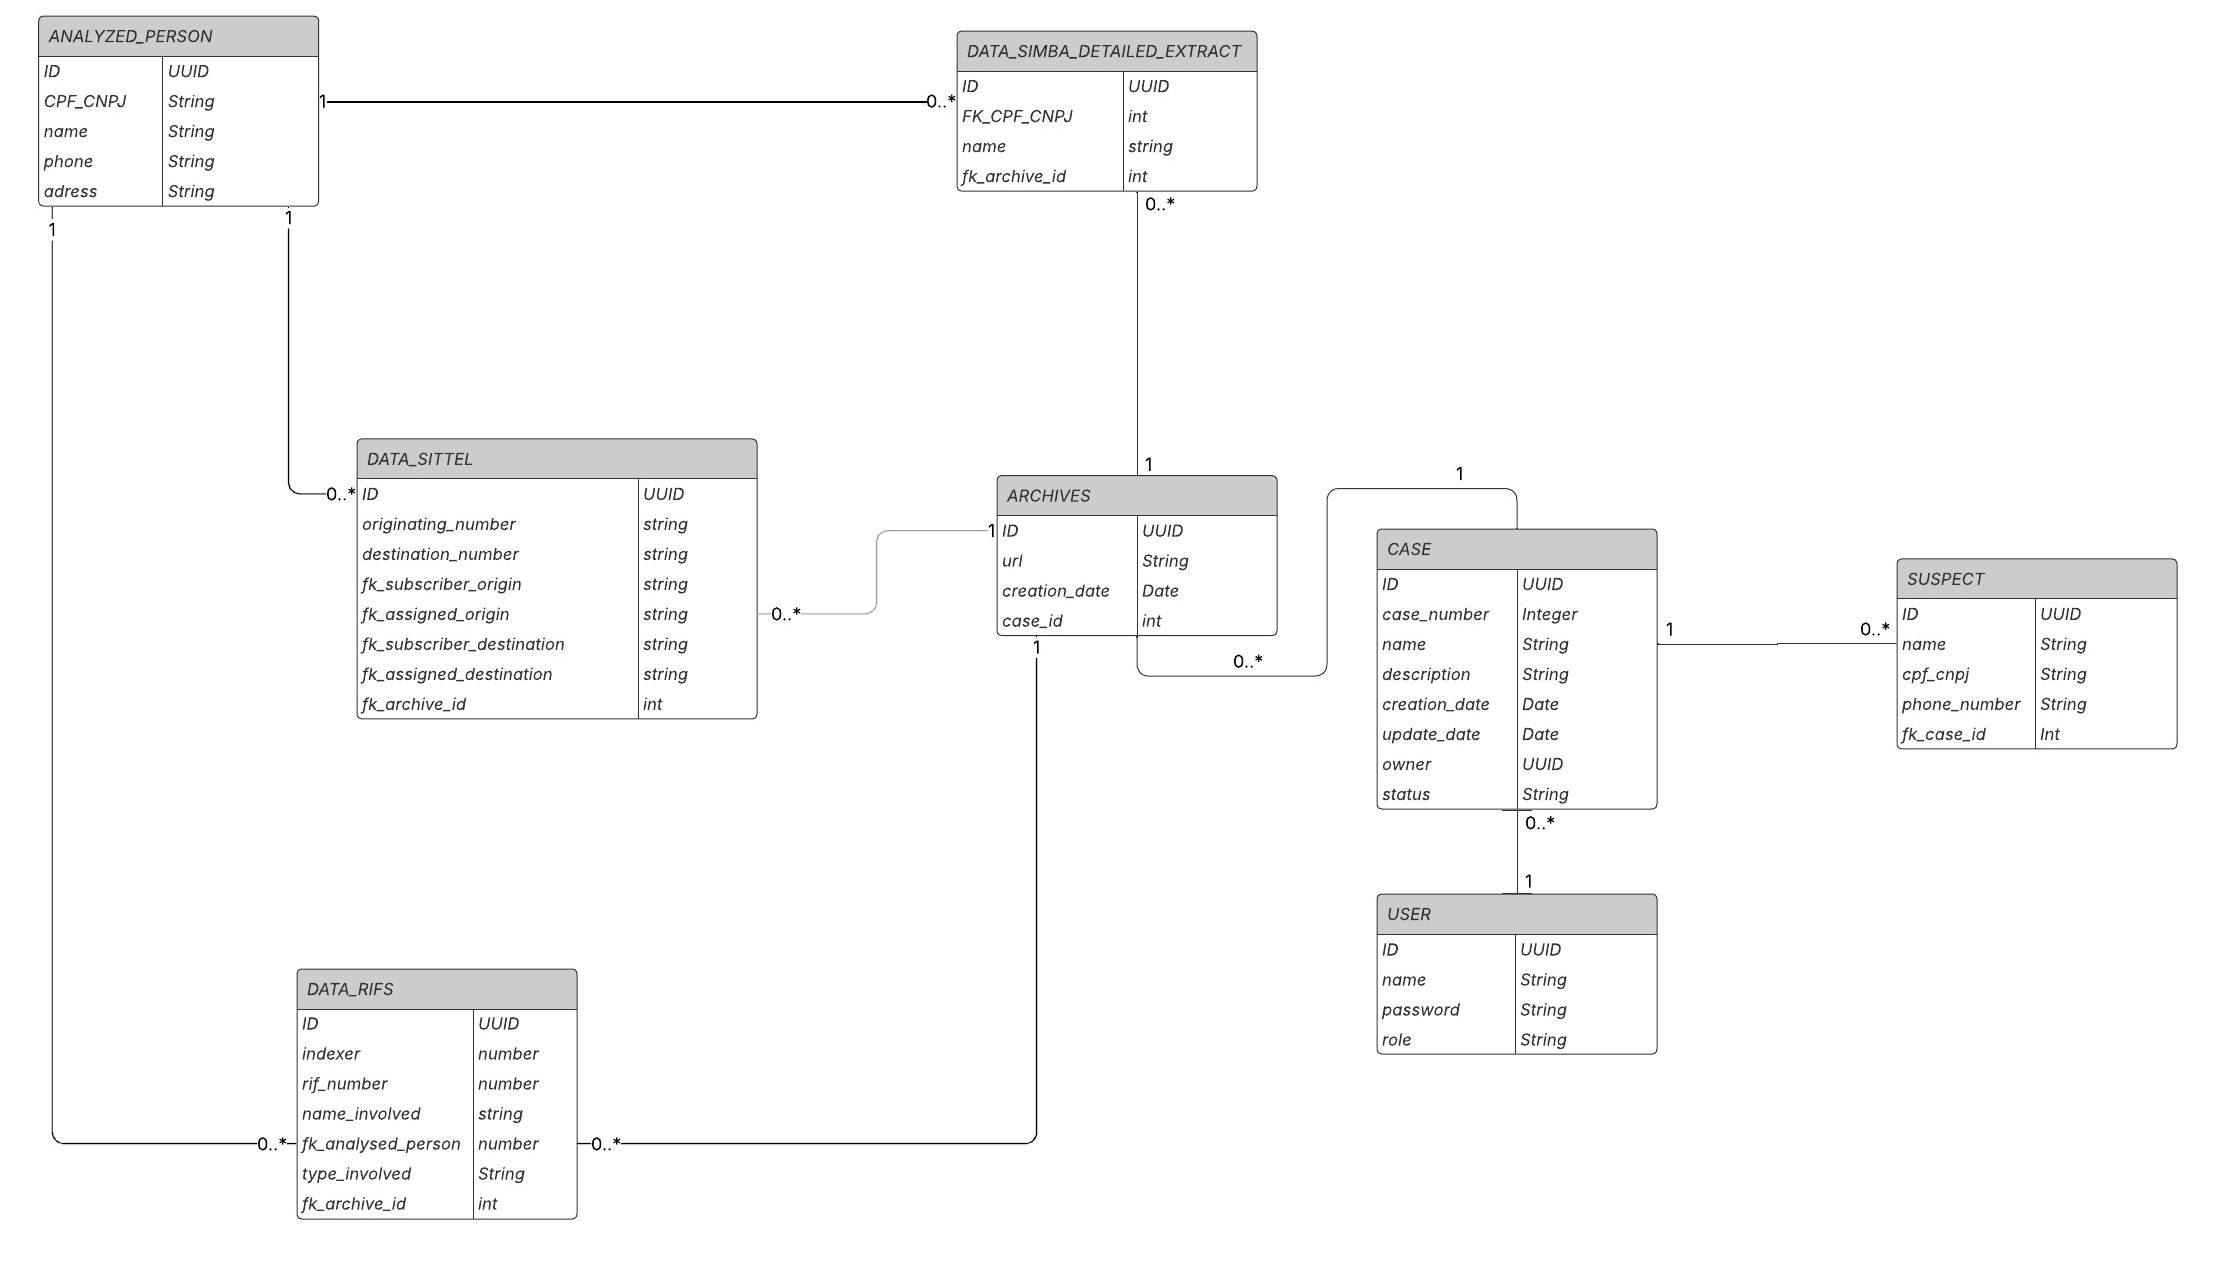
\includegraphics[width=1\linewidth]{conteudo//2 - ages I//conteudo//figures//banco-postgresql.jpeg}
    \caption{Modelo do banco relacional}
    Fonte: Adaptado de \textcites{wiki-vincula}
    \label{fig:modelo-banco}
  \end{figure}

\newpage
\subsection{Arquitetura Utilizada}
  A arquitetura do projeto Vincula foi projetada para ser executada na nuvem da \ac{aws} \cite{aws}, utilizando uma combinação de serviços gerenciados e um ambiente containerizado para garantir eficiência e automação no ciclo de desenvolvimento. A \autoref{fig:diagrama-deploy} mostra o diagrama de Deploy na \acs{aws}.

  \begin{figure}[H]
    \centering
    \small
    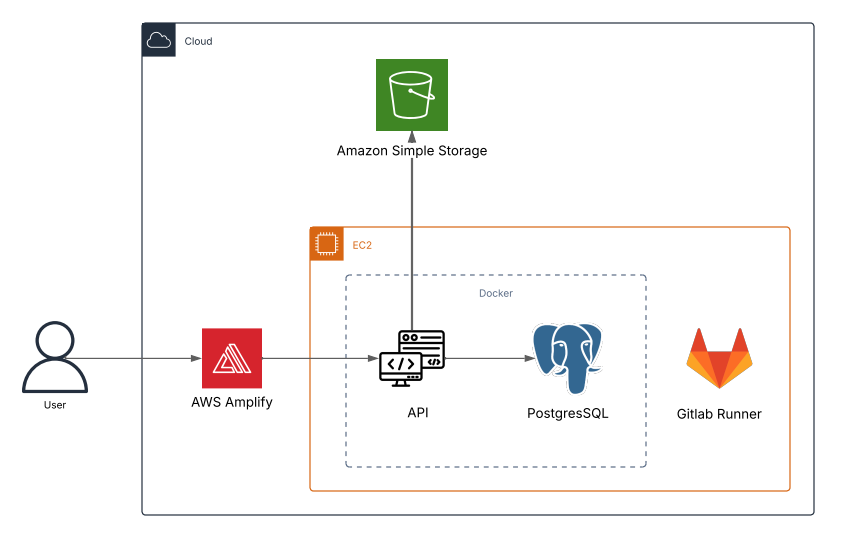
\includegraphics[width=1\linewidth]{conteudo//2 - ages I//conteudo//figures//arquitetura.png}
    \caption{Diagrama de Deploy}
    Fonte: Adaptado de \textcites{wiki-vincula}
    \label{fig:diagrama-deploy}
  \end{figure}

  Conforme ilustrado pelo diagrama da \autoref{fig:diagrama-deploy}, a arquitetura da solução segue um fluxo claro e desacoplado. A interface com o usuário, hospedada no AWS Amplify \cite{amplify}, consome uma API backend em Python \cite{python} com FastAPI. Esta API, juntamente com o banco de dados PostgreSQL, opera de forma containerizada com Docker \cite{docker} em uma instância Amazon EC2 \cite{ec2}. O sistema é complementado pelo Amazon S3 \cite{s3}, responsável pelo armazenamento de arquivos, e por um GitLab Runner \cite{gitlabrunner} na mesma instância EC2, que automatiza o processo de integração e entrega contínua (CI/CD).

\subsection{Protótipos das Telas Desenvolvidas}
  Os protótipos para as telas centrais da aplicação foram desenvolvidos utilizando a ferramenta Figma \cite{figma}. O manual de identidade visual do \acs{mprs} foi usado como referência para cores, estilo e logomarcas. 
  
  Algumas das telas são: Tela de Autenticação (\autoref{fig:tela-login}), Tela de Listagem de Casos (\autoref{fig:tela-home}), Tela do Caso (\autoref{fig:tela-caso}) e a Tela de Visualização de Vínculos (\autoref{fig:tela-vinculos}).

  As demais telas estão disponíveis no Figma do projeto:
  
  \url{https://www.figma.com/design/mvL3UaJUd8Rnnctve1iSpV/Vincula-AGES}

  \begin{figure}[H]
    \centering
    \small
    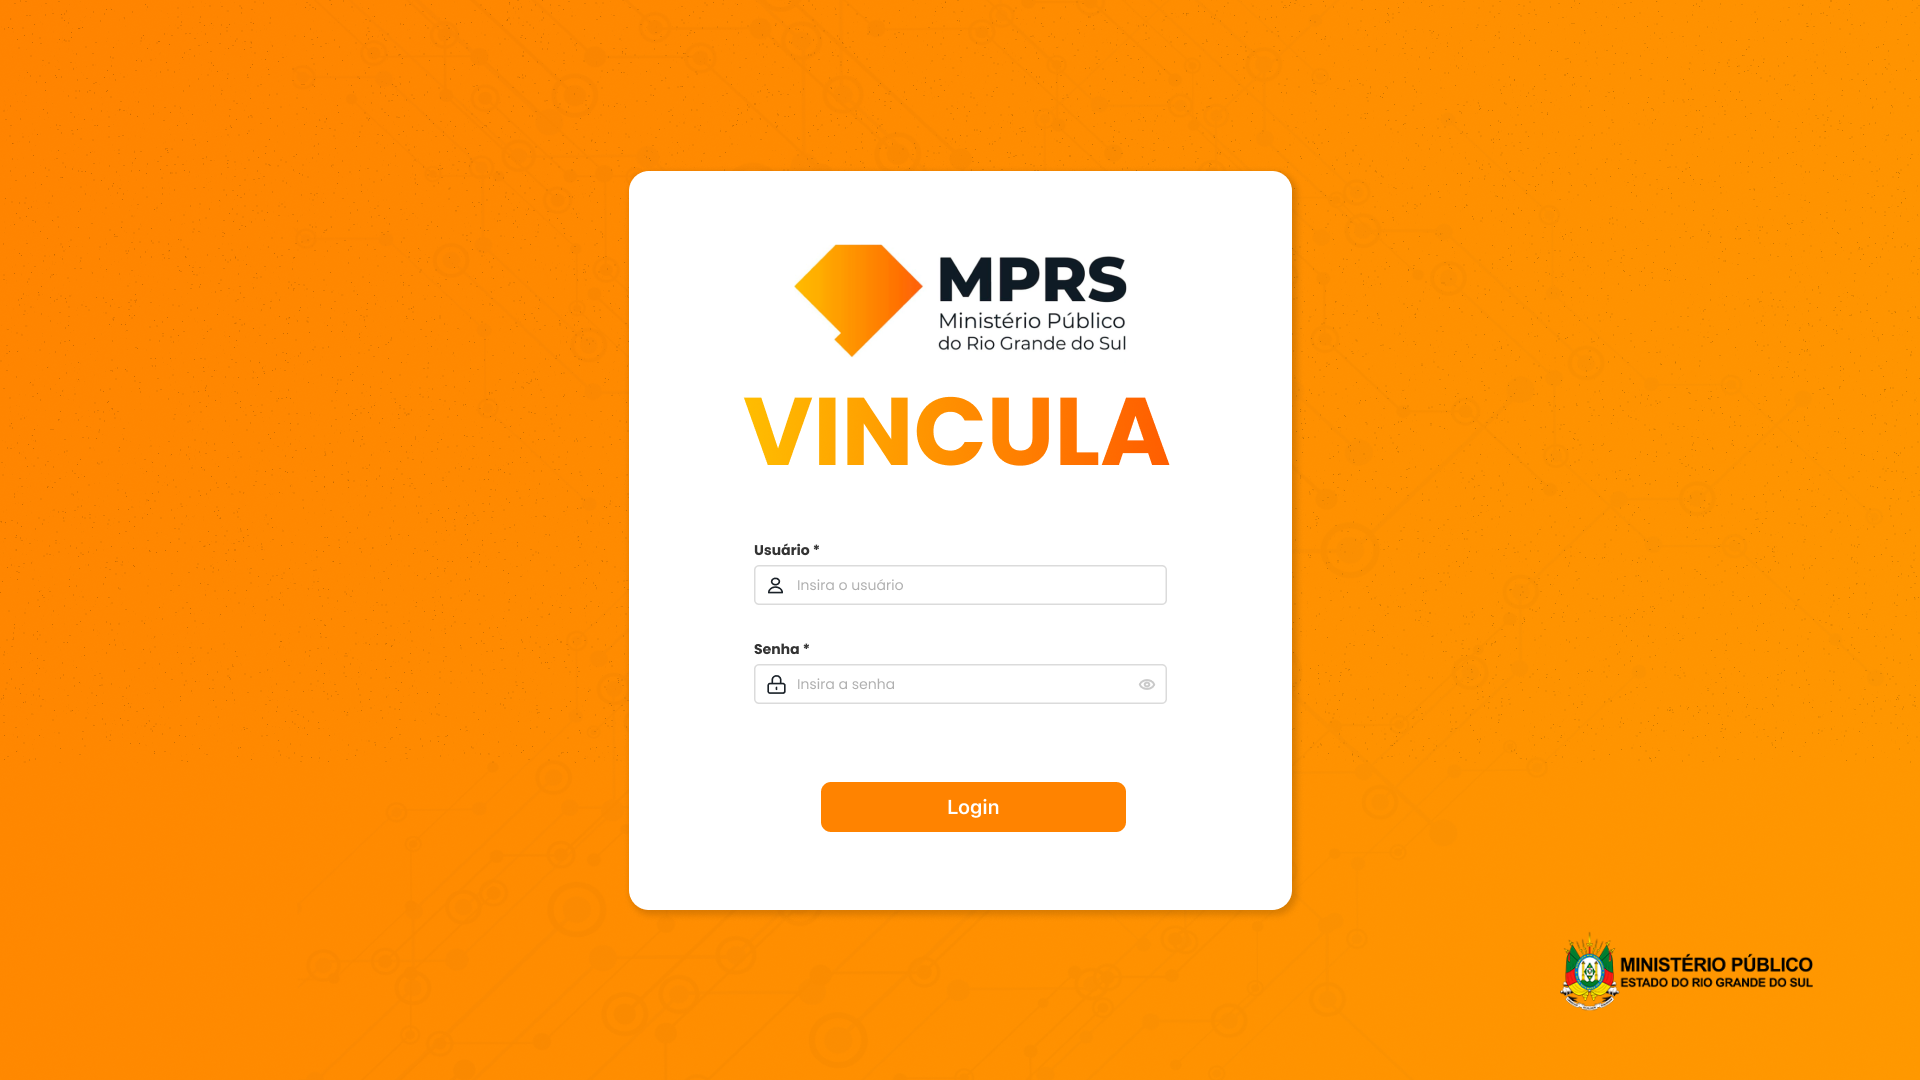
\includegraphics[width=1\linewidth]{conteudo//2 - ages I//conteudo//figures//tela-login.png}
    \caption{Tela de Autenticação}
    Fonte: Adaptado de \textcites{figma-vincula}
    \label{fig:tela-login}
  \end{figure}

  \begin{figure}[H]
    \centering
    \small
    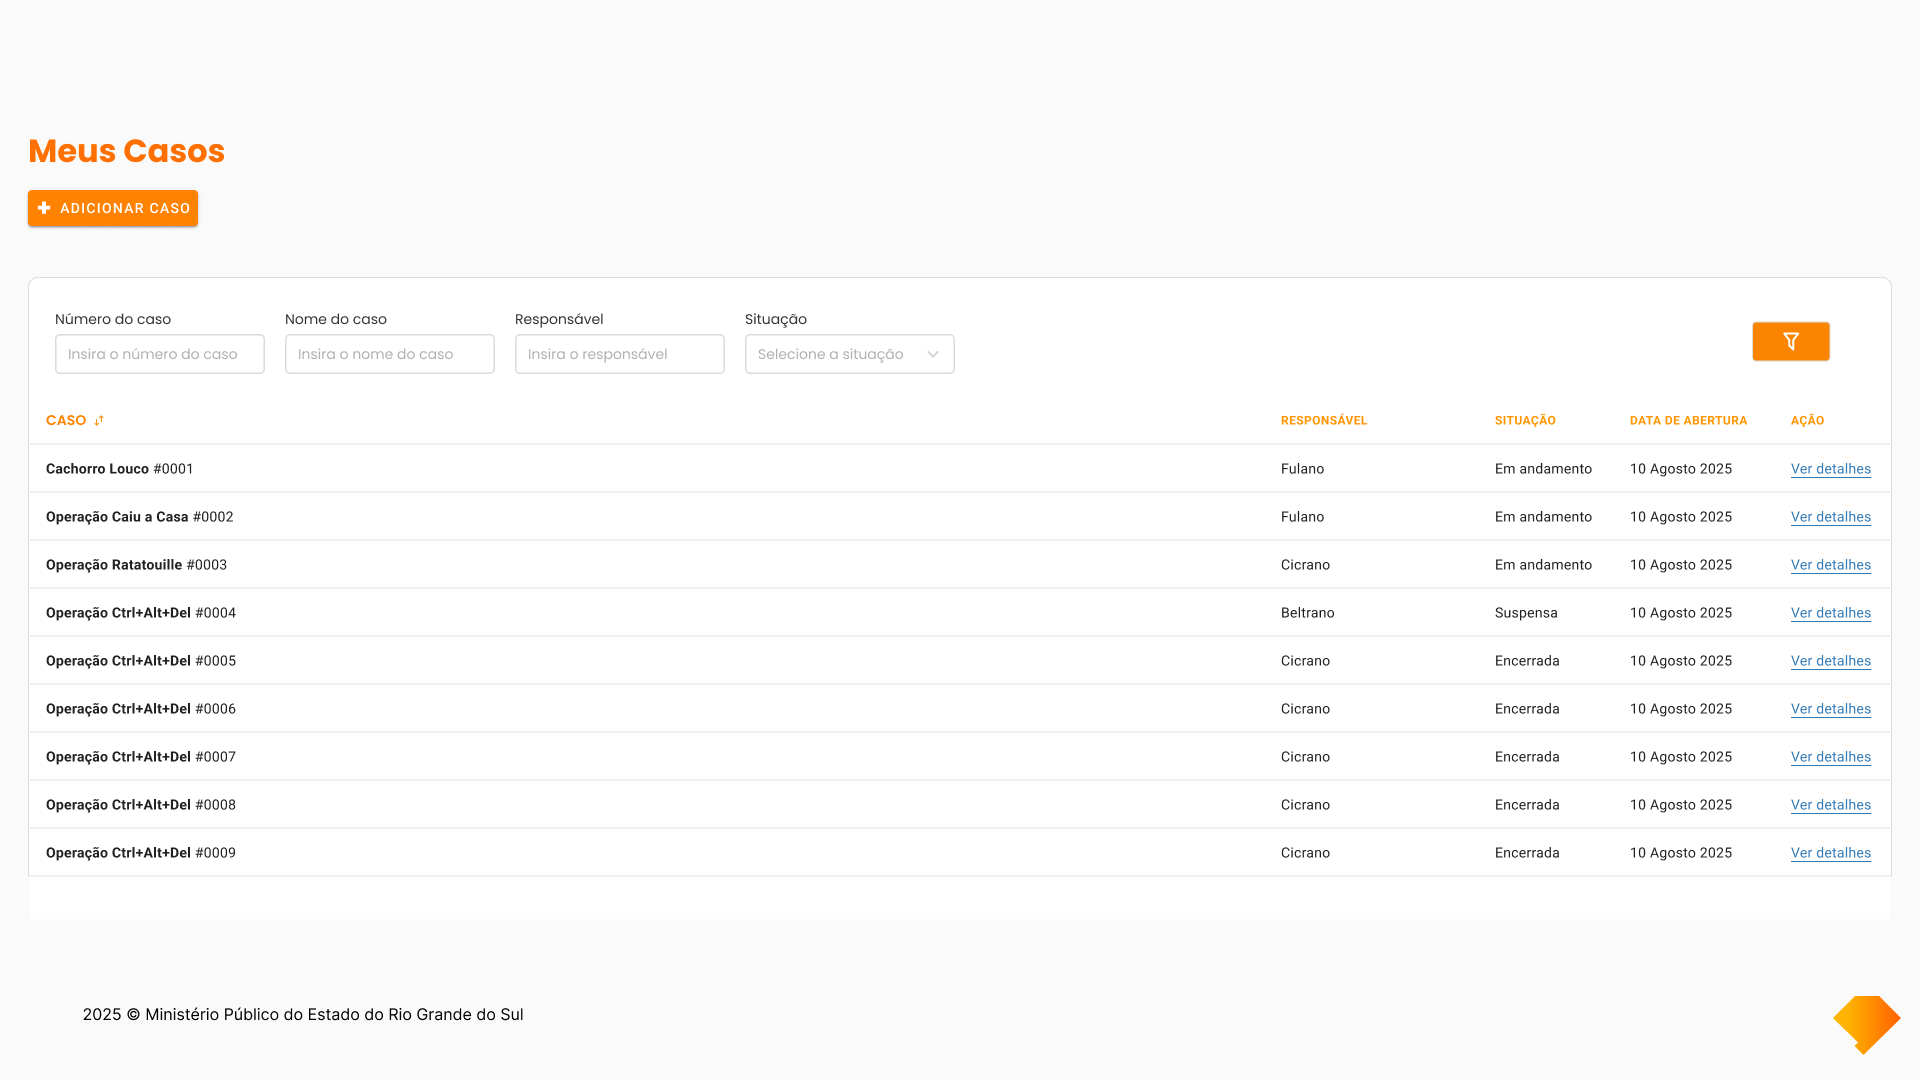
\includegraphics[width=1\linewidth]{conteudo//2 - ages I//conteudo//figures//tela-home.png}
    \caption{Tela de Listagem de Casos}
    Fonte: Adaptado de \textcites{figma-vincula}
    \label{fig:tela-home}
  \end{figure}

  \begin{figure}[H]
    \centering
    \small
    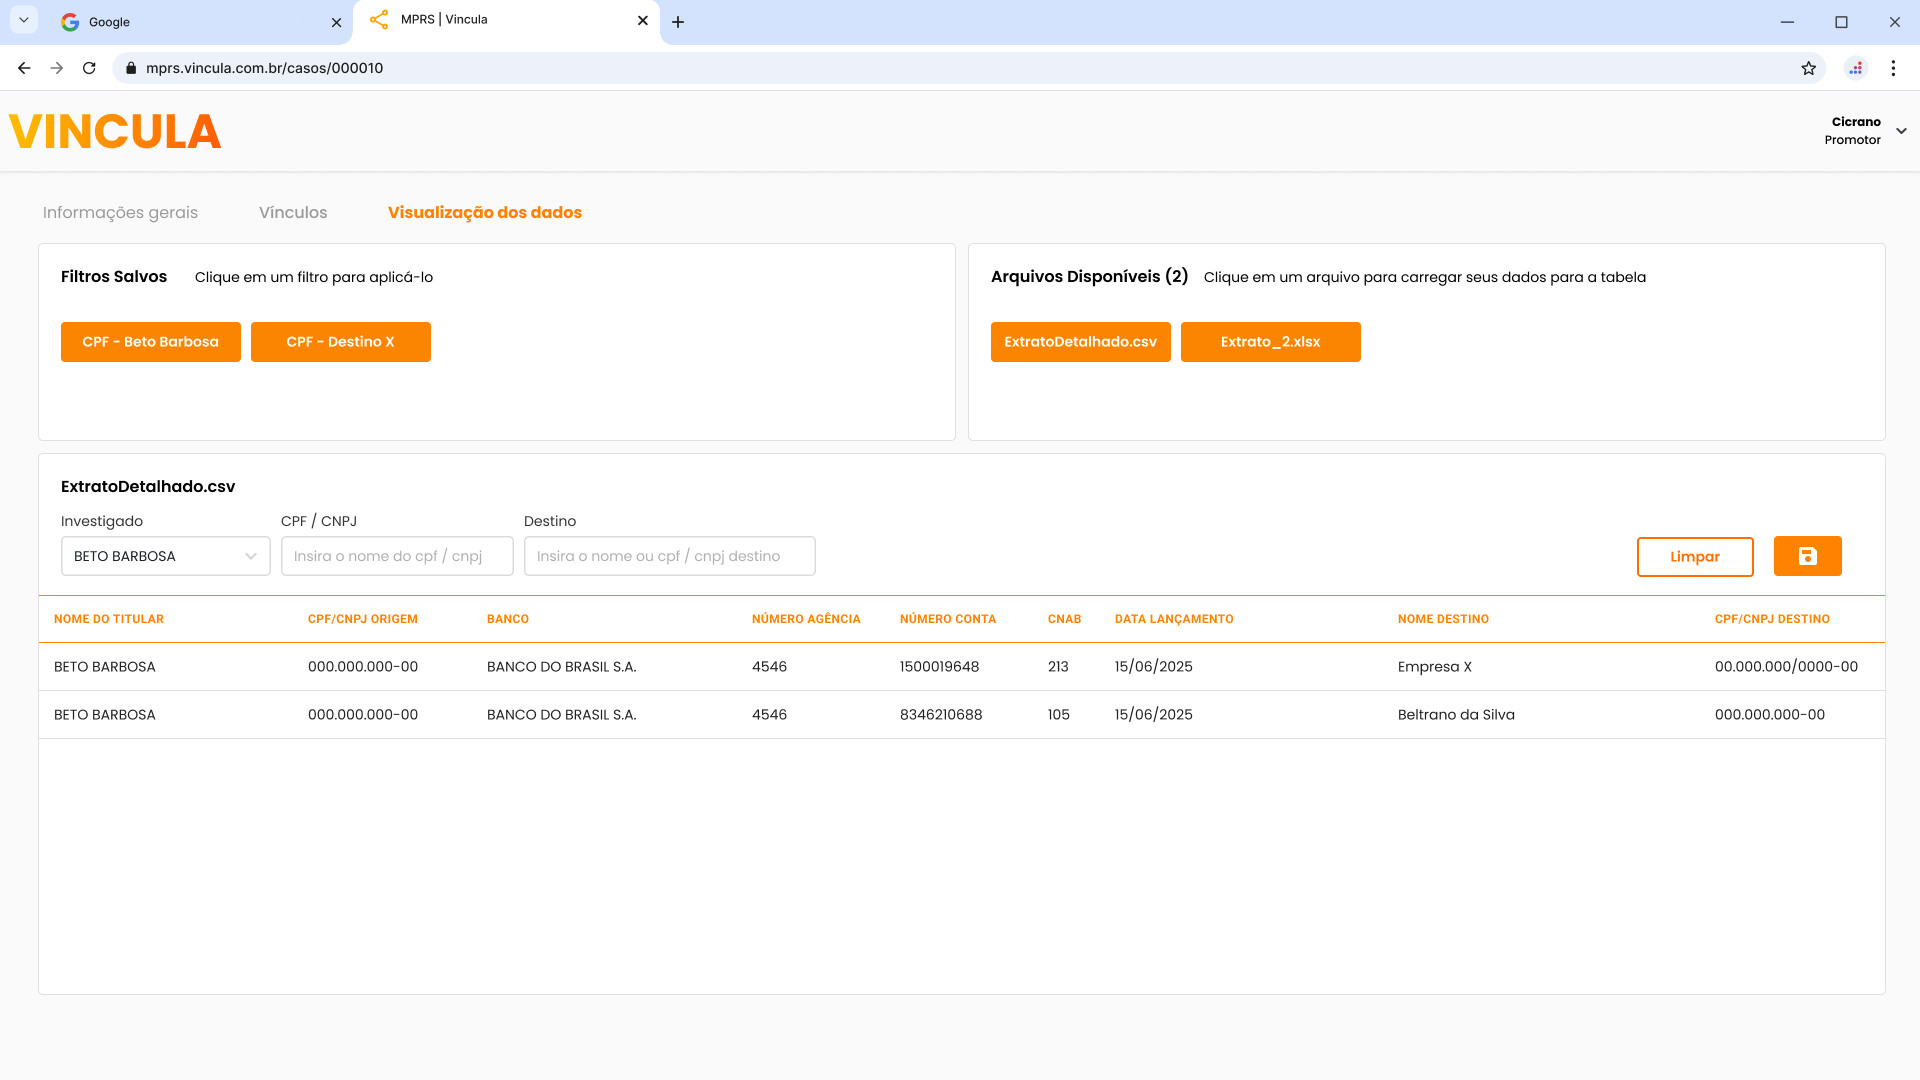
\includegraphics[width=1\linewidth]{conteudo//2 - ages I//conteudo//figures//tela-caso.png}
    \caption{Tela do Caso}
    Fonte: Adaptado de \textcites{figma-vincula}
    \label{fig:tela-caso}
  \end{figure}

  \begin{figure}[H]
    \centering
    \small
    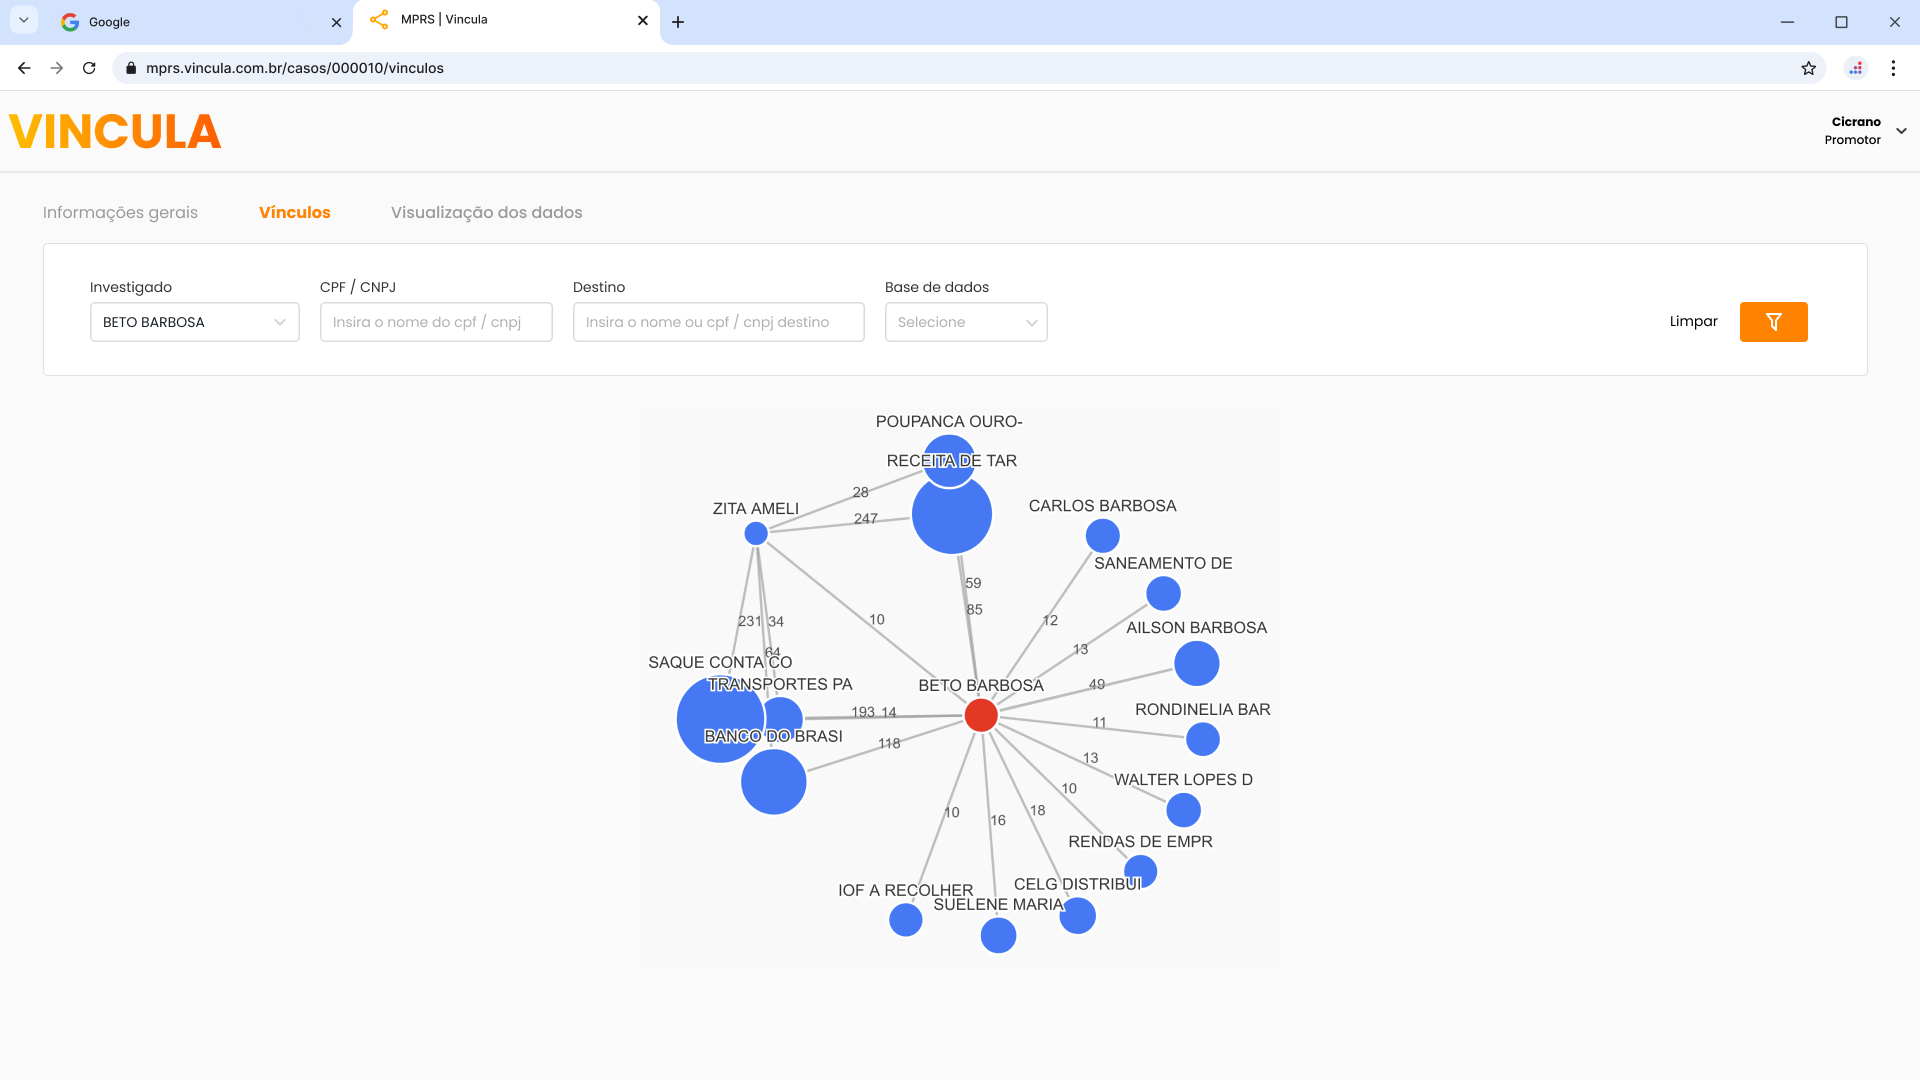
\includegraphics[width=1\linewidth]{conteudo//2 - ages I//conteudo//figures//tela-vinculos.png}
    \caption{Tela de Visualização de Vínculos}
    Fonte: Adaptado de \textcites{figma-vincula}
    \label{fig:tela-vinculos}
  \end{figure}

\subsection{Tecnologias Utilizadas}
  O projeto é construido utilizando quatro tecnologias principais, sendo elas o React \cite{react} com NextJs \cite{nextjs} e a linguagem TypeScript \cite{typescript} para o frontend, o FastAPI \cite{fastapi}, com a linguagem Python para o backend, PostgreSQL para o banco relacional e Neo4j \cite{neo4j} para o banco de grafos.
  
  O NextJs foi escolhido para o frontend por ser uma framework moderna e que abstrai diversos aspectos trabalhosos do desenvolvimento com a biblioteca React pura.

  No backend, logo de início, decidimos que uma framework Python seria essencial para o projeto, visto a necessidade de manipular grandes volumes de dados de forma eficiênte. Por isso, optamos pela FastAPI, que torna o processo de programar endpoints simplificado. O processamento de dados será feito com a biblioteca Pandas \cite{pandas}.

  O gerenciamento de tarefas, o planejamento das sprints e o controle do backlog são realizados na plataforma Azure DevOps. O controle de versão é feito com Git, hospedado no servidor da \acs{ages}. Todo o ambiente de desenvolvimento é containerizado com Docker.